\documentclass[paper=letter,fontsize=11pt]{scrartcl} % KOMA-article class
\usepackage[english]{babel}
\usepackage[utf8x]{inputenc}
\usepackage[protrusion=true,expansion=true]{microtype}
\usepackage{amsmath,amsfonts,amsthm}     % Math packages
\usepackage{graphicx}                    % Enable pdflatex
\usepackage[svgnames]{xcolor}            % Colors by their 'svgnames'
\usepackage{geometry}
	%\textheight=700px                    % Saving trees ;-)
%\usepackage{url}
\usepackage[colorlinks=true,
linkcolor=blue,
urlcolor=blue]{hyperref}
\usepackage{float}
\usepackage{etaremune}
\usepackage{wrapfig}
\usepackage{framed,graphicx,xcolor}
\definecolor{shadecolor}{rgb}{0.85,0.85,1}

\usepackage{attachfile}

\frenchspacing              % Better looking spacings after periods
\pagestyle{empty}           % No pagenumbers/headers/footers

%\addtolength{\voffset}{-40pt}
%\addtolength{\textheight}{20pt}

\setlength\topmargin{0pt}
\addtolength\topmargin{-\headheight}
\addtolength\topmargin{-\headsep}
\setlength\oddsidemargin{0pt}
\setlength\textwidth{\paperwidth}
\addtolength\textwidth{-2in}
\setlength\textheight{\paperheight}
%\addtolength\textheight{-3in}
\addtolength\textheight{-2in}
\usepackage{layout}

%%% Custom sectioning}{sectsty package)
%%% ------------------------------------------------------------
\usepackage{sectsty}

\sectionfont{%			            % Change font of \section command
	\usefont{OT1}{phv}{b}{n}%		% bch-b-n: CharterBT-Bold font
	\sectionrule{0pt}{0pt}{-5pt}{3pt}}

%%% Macros
%%% ------------------------------------------------------------
\newlength{\spacebox}
\settowidth{\spacebox}{8888888888}			% Box to align text
\newcommand{\sepspace}{\vspace*{0.75em}}		% Vertical space macro

\newcommand{\MyName}[1]{ % Name
		\Huge \usefont{OT1}{phv}{b}{n} \hfill #1
		\par \normalsize \normalfont}

\newcommand{\MySlogan}[1]{ % Slogan}{optional)
		\large \usefont{OT1}{phv}{m}{n}\hfill \textit{#1}
		\par \normalsize \normalfont}

\newcommand{\NewPart}[2]{\section*{\uppercase{#1} #2}}

\newcommand{\PersonalEntry}[2]{
		\noindent\hangindent=2em\hangafter=0 % Indentation
		\parbox{\spacebox}{        % Box to align text
		\textit{#1}}		       % Entry name}{birth, address, etc.)
		\hspace{1.5em} #2 \par}    % Entry value

\newcommand{\SkillsEntry}[2]{      % Same as \PersonalEntry
		\noindent\hangindent=2em\hangafter=0 % Indentation
		\parbox{\spacebox}{        % Box to align text
		\textit{#1}}			   % Entry name}{birth, address, etc.)
		\hspace{1.5em} #2 \par}    % Entry value

\newcommand{\EducationEntry}[4]{
		\noindent \textbf{#1} \hfill      % Study
		\colorbox{White}{%
			\parbox{10em}{%
			\hfill\color{Black}#2}} \par  % Duration
		\noindent \textit{#3} \par        % School
		\noindent\hangindent=2em\hangafter=0 \small #4 % Description
		\normalsize \par}

\newcommand{\WorkEntry}[4]{				  % Same as \EducationEntry
		\noindent \textbf{#1} \hfill      % Jobname
		\colorbox{White}{\color{White}#2} \par  % Duration
		\noindent \textit{#3} \par              % Company
		\noindent\hangindent=2em\hangafter=0 \small #4 % Description
		\normalsize \par}

\newcommand{\PaperEntry}[7]{
		\noindent #1, ``\href{#7}{#2}", \textit{#3} \textbf{#4}, #5 (#6).}


\newcommand{\ArxivEntry}[3]{
		\noindent #1, ``\href{http://arxiv.org/abs/#3}{#2}", \textit{{cond-mat/}#3}.}

\newcommand{\BookEntry}[4]{
		\noindent #1, ``\href{#3}{#4}", \textit{#3}.}

\newcommand{\FundingEntry}[5]{
        \noindent #1, ``#2", \$#3 (#4, #5).}

\newcommand{\TalkEntry}[4]{
		\noindent #1, #2, #3 #4}

\newcommand{\ThesisEntry}[5]{
		\noindent #1 -- #2 #3 ``#4" \textit{#5}}

\newcommand{\CourseEntry}[3]{
		\noindent \item{#1: \textbf{#2} \\ #3}}

%%% Begin Document
%%% ------------------------------------------------------------
\begin{document}

%\layout

% you can upload a photo and include it here...
\begin{wrapfigure}{l}{0.5\textwidth}
	\vspace*{-2em}
		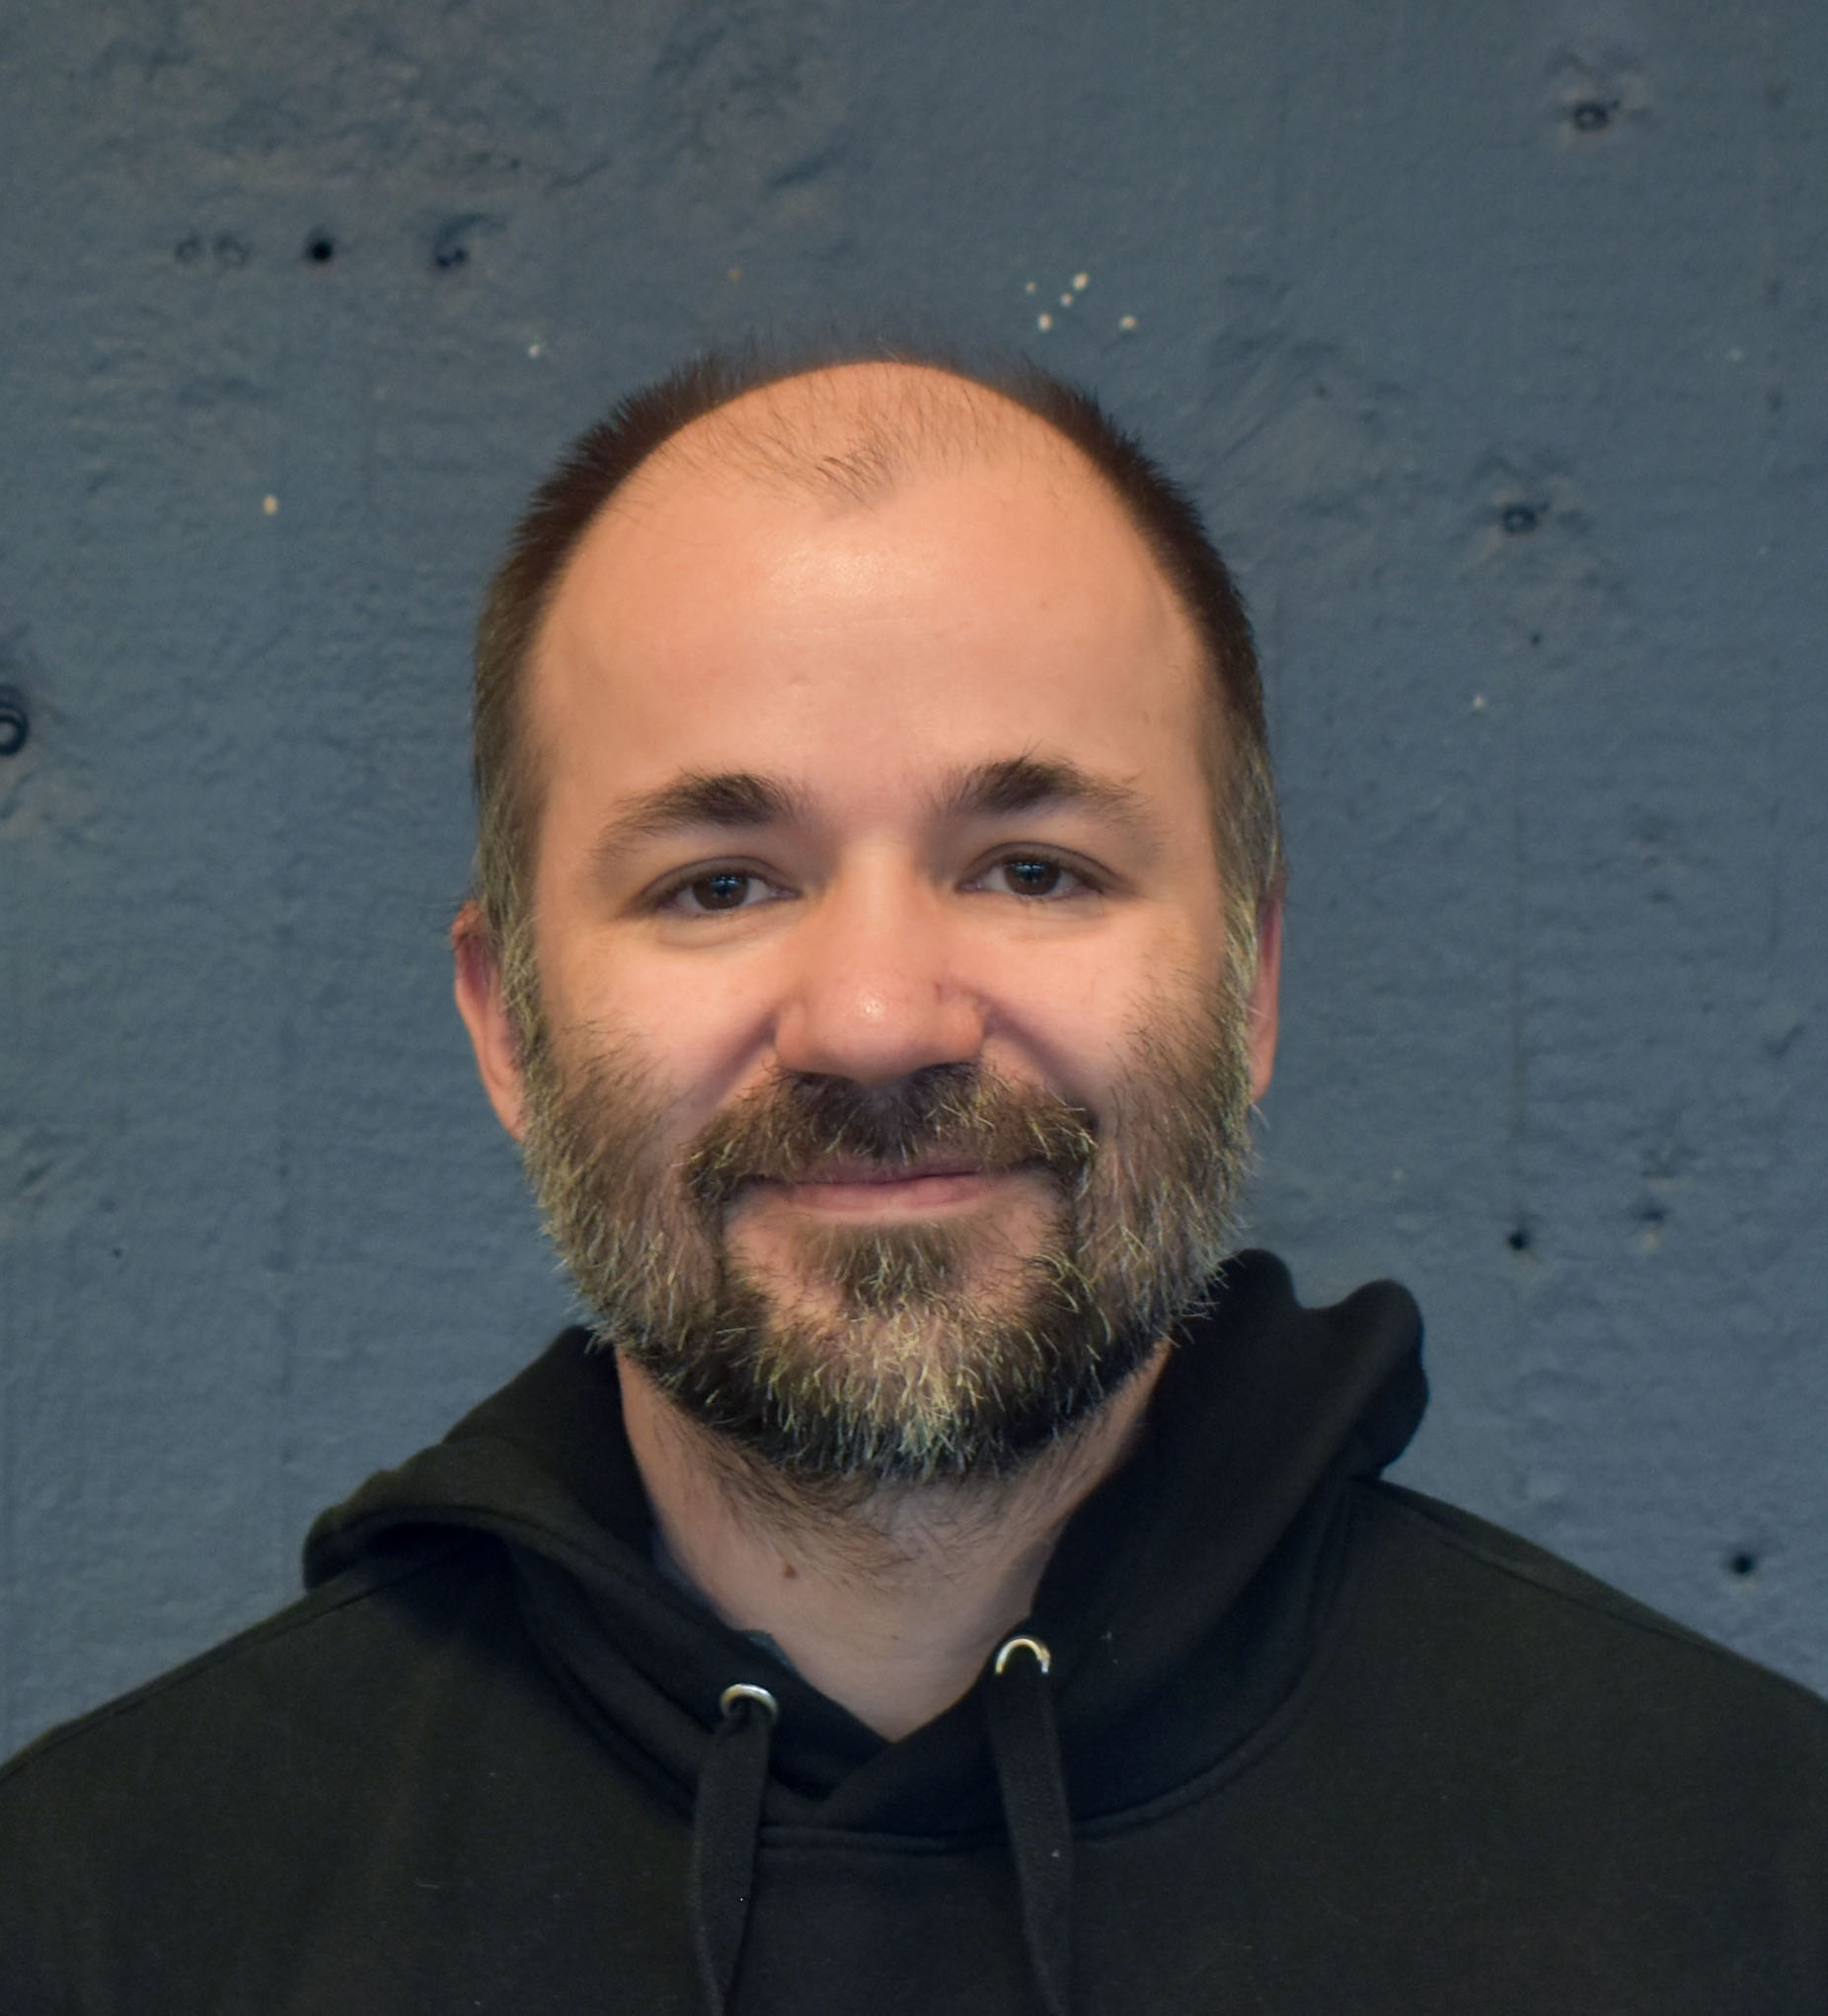
\includegraphics[width=0.15\textwidth]{wasp_profile.jpg}
\end{wrapfigure}

\MyName{Philipp Leitner}
\MySlogan{Curriculum Vit\ae\ (\today)}

\sepspace

%%% Personal details
%%% ------------------------------------------------------------
\NewPart{}{}

\PersonalEntry{Address}{Hörselgången 5,
  417 56 Göteborg, Sweden}
\PersonalEntry{Phone}{+41 44 63 545 81}
\PersonalEntry{Mail}{\href{mailto:philipp.leitner@chalmers.se}{philipp.leitner@chalmers.se}}
\PersonalEntry{WWW}{\href{http://philippleitner.net}{http://philippleitner.net}}

\NewPart{Summary}{}
I am an Associate Professor (Docent) of Software Engineering at Chalmers and the University of Gothenburg, Sweden, where I lead the Internet Computing and Emerging Technologies (ICET) research lab. I hold a PhD degree from Vienna University of Technology. My primary research interest is empirical software engineering, with a particular focus on software performance, developer tooling, and the development of Web- and cloud-based systems. I have published around 125 peer-reviewed publications, leading to an h-index of 46 as tracked by Google Scholar.


%%% Education
%%% ------------------------------------------------------------
\NewPart{Education}{}

\EducationEntry{Oavlönad Docent in Software Engineering}{Jun. 2019}{Chalmers University of Technology}{}

\EducationEntry{PhD Business Informatics}{Oct. 2007 - Oct. 2011}{Vienna
University of Technology}{}

%%% Work experience
%%% ------------------------------------------------------------
\NewPart{Appointments and Work History}{}

\EducationEntry{Associate Professor}{Since Oct. 19}{Chalmers $|$ University of Gothenburg}{}
\EducationEntry{Assistant Professor}{Aug. 17 - Oct. 19}{Chalmers $|$ University of Gothenburg}{}
\EducationEntry{Senior Research Associate}{Jan. 2014 - Jul. 2017}{University of
Zurich}{}
\EducationEntry{Postdoctoral Researcher}{Nov. 2011 - Dec. 2013}{Vienna
University of Technology}{}
\EducationEntry{Research and Teaching Assistant}{Oct. 2007 - Oct. 2011}{Vienna
University of Technology} {}
\EducationEntry{Research Software Engineer}{Jul. 2005 - Sep. 2007}{Siemens PSE,
Vienna}{}

\newpage

\NewPart{Selected Grants}{}

I have successfully acquired grants (personal as well as project grants) totalling around 28 MSEK. Selected list:

\begin{itemize}
  \itemsep0em 
  \item 3x WASP Academic PhD Student (2017-2030)\\
  Academic Supervisor\\
  Grant value $>$10,000,000 SEK  
  \item FFI TrafCloud (2019 -- 2021), VINNOVA\\
	Co-applicant\\
	Chalmers budget 5,500,000 SEK (my part $\approx$3,200,000 SEK)
  \item VR Starting Grant (2019 -- 2022), VR\\
  Sole applicant\\
	Grant value 3,639,000 SEK
  \item Individual Project (2016 -- 2019), Swiss National Science Foundation\\
  Sole applicant \\
  Grant value 180,000 CHF, at University of Zurich
\end{itemize}

\NewPart{Selected Talks}{}

\begin{itemize}
  \itemsep0em 
  \item \emph{A Brief Journey Through History - From Distributed Objects over SOA to Microservices}, Two opening keynotes at CLOSER and ICEIS, April 2025
  \item \emph{Measuring, Predicting, and Improving the Performance of Software Systems}, Invited Talk at the Department Colloquium, Institute for Informatics, University of Zurich, November 2024
  \item \emph{Unit testing performance using code microbenchmarks. How far are we?}, Invited Talk at MongoDB Inc., November 2020
	\item \emph{Performance stability of (public) clouds}, Invited Talk at Vehicle Electronics and Connected Services (VECS, industrial conference), April 2019
	tem \emph{Predictability of Performance in Public Clouds - Some Empirical Data and Lessons Learned for Software Performance Testing}, Seminar at IBM Research, Ireland, November 2017
\item \emph{How Predictable is the Performance of IaaS Instances? Some Insights from Benchmarking EC2, GCE, Azure, and Softlayer}, Open Cloud Day, ZHAW Winterthur, June 2016
\item \emph{Trends, Opportunities and Challenges of Software Development for the Cloud}, Two talks at Indian Institute of Technology New Delhi and Ropar, by invitation of the Swiss Embassy in India, November 2015
\end{itemize}

\NewPart{Selected Awards}{}
\begin{itemize}
\itemsep0em 
\item Distinguished Reviewer Award (ICSE 2023)   
\item Distinguished Reviewer Award (MSR 2020)
\item Outstanding Reviewer Award (ICPE 2019 and 2020)
\item Best Student Paper Award (Middleware 2016)
\item Best Short Paper Award (ICPC 2016)
\end{itemize}

\NewPart{Selected Service}{}
\begin{itemize}
  \itemsep0em 
\item Associate Editor of Springer Empirical Software Engineering (EMSE)
\item Academic Editor of PeerJ Computer Science (until 2024)
\item Chair of the Selection Committee of the 2022 SPEC Kaivalya Dixit Distinguished Dissertation Award 
\item Program Co-Chair of 13th ACM/SPEC International Conference on Performance Engineering (ICPE) 
\item Editorial Board Member of Elsevier's Journal on Systems and Software (JSS). Responsible for coordinating and implementing the publicity efforts of the journal. 2017 - 2019.
\item General Chair of the 1st International Workshop on Monitoring and
Prediction of Cloud Services (MoPoC'12), co-located with ICSOC'12.
\item Various PC memberships, including ICSE 2023, FSE 2024 and 2025, ASE 2022 and 2024, CLOUD (various years), ICPE (various years), and MSR (various years).
\end{itemize}

\NewPart{PhD Students}{}

\begin{itemize}
  \itemsep0em   
\item \textbf{Lirong (Esme) Yi} (Optimizing Performance using Large Language Models)
\item \textbf{Ranim Khojah} (Large Language Models in Software Engineering, \emph{co-supervisor})
\item \textbf{Huaifeng Zhang}  (Debloating ML Systems, \emph{co-supervisor})  
\item \textbf{Linda Erlenhov}  (Bots in Software Development)
\item \textbf{Hazem (Peter) Samoaa}  (graduated at Chalmers, ML for Performance Prediction)
\item \textbf{Hamdy Michael Ayas}  (graduated at Chalmers, Architectural Decision Making in Cloud Computing, now consultant at ICTech, Sweden)
\item \textbf{Joel Scheuner}  (graduated at Chalmers, Cloud Benchmarking, now software engineer at LocalStack, Switzerland)
\item \textbf{Christoph Laaber} (graduated at UZH, microbenchmarking in CI builds, co-supervised with Harald C. Gall, now postdoc at Simula, Norway)
\item \textbf{Gerald Schermann} (graduated at UHZ, continuous experimentation, co-supervised with Harald C. Gall, now release engineer at digitec.ch, Switzerland)
\item \textbf{J\"urgen Cito} (graduated at UZH, cloud performance engineering, co-supervised with Harald C. Gall, now Associate Professor at TU Wien, Austria)
\end{itemize}

\NewPart{Selected Papers}{}

I have published around 125 peer-reviewed publications, leading to an h-index of 46. A full list is available on Google Scholar: \href{https://scholar.google.ch/citations?user=wZ9f8CAAAAAJ}{link}.

\begin{itemize}
  \itemsep0em
  \item  R. Khojah, M. Mohamad, \textbf{P. Leitner}, and F. Gomes: Beyond Code Generation: An Observational Study of ChatGPT Usage in Software Engineering Practice. Proceedings of the ACM International Conference on the Foundations of Software Engineering (FSE). 2024.
  \item H. Zhang, M. Alhanahnah, F. Ahmed, D. Fatih, \textbf{P. Leitner} and A. Ali-Eldin: \emph{Machine Learning systems are Bloated and Vulnerable}, in Proceedings of the ACM International Conference on Measurement and Modeling of Computer Systems (SIGMETRICS). 2024.    
  \item H. M. Ayas, \textbf{P. Leitner}, and R. Hebig: \emph{An Empirical Study of the Systemic and Technical Migration Towards Microservices}, Empirical Software Engineering (EMSE), 2023.
  \item M. Jangali, Y. Tang, N. Alexandersson, \textbf{P. Leitner}, J. Yang, and W. Shang: \emph{Automated Generation and Evaluation of JMH Microbenchmark Suites from Unit Tests}, IEEE Transactions on Software Engineering (TSE), 2022.
  \item P. Samoaa and \textbf{P. Leitner}: \emph{An Exploratory Study of the Impact of Parameterization on JMH Measurement Results in Open-Source Projects}, in Proceedings of the ACM/SPEC  International Conference on Performance Engineering (ICPE). 2021.    
  \item C. Laaber, \textbf{P. Leitner}, and H. Gall: \emph{Applying Test Case Prioritization to Software Microbenchmarks}, Empirical Software Engineering (EMSE), 26, 133 (2021).
\item C. Laaber,  S. Würsten, H. C. Gall, and \textbf{P. Leitner}: \emph{Dynamically Reconfiguring Software Microbenchmarks: Reducing Execution Time Without Sacrificing Result Quality}, in Proceedings of the ACM Joint European Software Engineering Conference and Symposium on the Foundations of Software Engineering (ESEC/FSE). 2020.
\item L. Erlenhov,  F. Gomes, and \textbf{P. Leitner}: \emph{An Empirical Study of Bots in Software Development - Characteristics and Challenges from a Practitioner's Perspective}, in Proceedings of the ACM Joint European Software Engineering Conference and Symposium on the Foundations of Software Engineering (ESEC/FSE). 2020.
  \item J. Cito, \textbf{P. Leitner}, M. Rinard, and H. C. Gall: \emph{Interactive Production Performance Feedback in the IDE}, in Proceedings of the 41st ACM/IEEE International Conference on Software Engineering (ICSE). 2019.
  \item D. Costa, CP. Bezemer, \textbf{P. Leitner}, and  A. Andrzejak: \emph{What’s Wrong With My Benchmark Results? Studying Bad Practices in JMH Benchmarks}, in IEEE Transactions on Software Engineering (TSE). 2019.
		\item  C. Laaber, J. Scheuner, and \textbf{P. Leitner}: \emph{Software Microbenchmarking in the Cloud. How Bad is it Really?}, Empirical Software Engineering (EMSE). 2019.
	\item \textbf{P. Leitner}, E. Wittern, J. Spillner, and W. Hummer: \emph{A Mixed-Method Empirical Study of Function-as-a-Service Software Development in Industrial Practice}, Journal of Systems and Software (JSS). 2019.
	\item  \textbf{P. Leitner} and J. Cito: \emph{Patterns in the Chaos -- a Study of Performance Variation and Predictability in Public IaaS Clouds}, ACM Transactions on Internet Technology (TOIT). 2016.
	\item G. Schermann, D. Schöni, \textbf{P. Leitner}, and H. C. Gall: \emph{Bifrost -- Supporting Continuous Deployment with Automated Enactment of Multi-Phase Live Testing Strategies}, in Proceedings of the ACM/IFIP/USENIX Middleware Conference. 2016.  
	\item J. Cito, \textbf{P. Leitner}, T. Fritz, and H. C. Gall: \emph{The Making of Cloud Applications -- An Empirical Study on Software Development for the Cloud}, in Proceedings of the 10th Joint Meeting of the European Software Engineering Conference and the ACM SIGSOFT International Symposium on Foundations of Software Engineering (ESEC/FSE). 2015.
\end{itemize}

\end{document}
